\documentclass[
    xcolor={svgnames,dvipsnames},
    hyperref={colorlinks, citecolor=DeepPink4, linkcolor=DarkRed, urlcolor=DarkBlue}
    ]{beamer}  % for hardcopy add 'trans'

\mode<presentation>
{
  \usetheme{Singapore}
  % or ...
  \setbeamercovered{transparent}
  % or whatever (possibly just delete it)
}



\addtobeamertemplate{navigation symbols}{}{%
    \usebeamerfont{footline}%
    \usebeamercolor[fg]{footline}%
    \hspace{1em}%
    \insertframenumber/\inserttotalframenumber
}



\usepackage{fontspec} 
%\usepackage[xcharter]{newtxmath}
%\setmainfont{XCharter}
\usepackage{unicode-math}
%\setmathfont{XCharter-Math.otf}
\setmonofont{DejaVu Sans Mono}[Scale=MatchLowercase] % provides unicode characters 

\usepackage{tikz}
\usetikzlibrary{matrix, shapes, arrows.meta, positioning, fit, backgrounds, calc}

% \usetikzlibrary{matrix, arrows.meta, positioning, calc, backgrounds}

% for tikz
\usepackage{pgfplots}
\usepgfplotslibrary{fillbetween}
\pgfplotsset{compat=1.16}

\usepackage{varwidth}
\usepackage{minted}
\usemintedstyle{friendly}
\setminted[python]{
  fontsize=\small,
  baselinestretch=1.2,
  bgcolor=codebg,
  linenos=false,
  breaklines=true,
  frame=none
}
\setminted[matlab]{
  fontsize=\small,
  baselinestretch=1.2,
  bgcolor=codebg,
  linenos=false,
  breaklines=true,
  frame=none
}
\setminted[julia]{
  fontsize=\small,
  baselinestretch=1.2,
  bgcolor=codebg,
  linenos=false,
  breaklines=true,
  frame=none
}
%\setminted{mathescape, frame=lines, framesep=3mm}
%\newminted{python}{}
%\newminted{c}{mathescape,frame=lines,framesep=4mm,bgcolor=bg}
%\newminted{java}{mathescape,frame=lines,framesep=4mm,bgcolor=bg}
%\newminted{julia}{mathescape,frame=lines,framesep=4mm,bgcolor=bg}
%\newminted{ipython}{mathescape,frame=lines,framesep=4mm,bgcolor=bg}

\usepackage{graphicx}
\usepackage{amsmath, amssymb, amsthm}
\usepackage{bbm}
\usepackage{mathrsfs}
\usepackage{xcolor}
\usepackage{fancyvrb}


% Quotes at start of chapters / sections
\usepackage{epigraph}  
\renewcommand{\epigraphwidth}{6in}

%% Fonts

%\usepackage[T1]{fontenc}
\usepackage{mathpazo}
%\usepackage{fontspec}
%\defaultfontfeatures{Ligatures=TeX}
%\setsansfont[Scale=MatchLowercase]{DejaVu Sans}
%\setmonofont[Scale=MatchLowercase]{DejaVu Sans Mono}
%\setmathfont{Asana Math}
%\setmainfont{Optima}
%\setmathrm{Optima}
%\setboldmathrm[BoldFont={Optima ExtraBlack}]{Optima Bold}

% Some colors

\definecolor{containerblue}{RGB}{66, 133, 244}
\definecolor{leafgreen}{RGB}{52, 168, 83}
\definecolor{textgray}{RGB}{51, 51, 51}
\definecolor{backgroundgray}{RGB}{248, 249, 250}
\definecolor{codebg}{RGB}{241, 241, 241}
\definecolor{aquamarine}{RGB}{69,139,116}
\definecolor{midnightblue}{RGB}{25,25,112}
\definecolor{darkslategrey}{RGB}{47,79,79}
\definecolor{darkorange4}{RGB}{139,90,0}
\definecolor{dogerblue}{RGB}{24,116,205}
\definecolor{blue2}{RGB}{0,0,238}
\definecolor{bg}{rgb}{0.95,0.95,0.95}
\definecolor{DarkOrange1}{RGB}{255,127,0}
\definecolor{ForestGreen}{RGB}{34,139,34}
\definecolor{DarkRed}{RGB}{139, 0, 0}
\definecolor{DarkBlue}{RGB}{0, 0, 139}
\definecolor{Blue}{RGB}{0, 0, 255}
\definecolor{Brown}{RGB}{165,42,42}


\setlength{\parskip}{1.5ex plus0.5ex minus0.5ex}

%\renewcommand{\baselinestretch}{1.05}
%\setlength{\parskip}{1.5ex plus0.5ex minus0.5ex}
%\setlength{\parindent}{0pt}

% Typesetting code
\definecolor{bg}{rgb}{0.95,0.95,0.95}
\newcommand{\Fact}{\textcolor{Brown}{\bf Fact. }}
\newcommand{\Facts}{\textcolor{Brown}{\bf Facts }}
\newcommand{\keya}{\textcolor{turquois4}{\bf Key Idea. }}
\newcommand{\Factnodot}{\textcolor{Brown}{\bf Fact }}
\newcommand{\Eg}{\textcolor{ForestGreen}{Example. }}
\newcommand{\Egs}{\textcolor{ForestGreen}{Examples. }}
\newcommand{\Ex}{{\bf Ex. }}



\renewcommand{\theFancyVerbLine}{\sffamily
    \textcolor[rgb]{0.5,0.5,1.0}{\scriptsize {\arabic{FancyVerbLine}}}}

\newcommand{\navy}[1]{\textcolor{DarkBlue}{\bf #1}}
\newcommand{\brown}[1]{\textcolor{Brown}{\sf #1}}
\newcommand{\green}[1]{\textcolor{ForestGreen}{\sf #1}}
\newcommand{\blue}[1]{\textcolor{Blue}{\sf #1}}
\newcommand{\emp}[1]{\textcolor{DarkOrange1}{\bf #1}}
\newcommand{\red}[1]{\textcolor{Red}{\bf #1}}

% Symbols, redefines, etc.

\newcommand{\code}[1]{\texttt{#1}}

\newcommand{\argmax}{\operatornamewithlimits{argmax}}
\newcommand{\argmin}{\operatornamewithlimits{argmin}}

\DeclareMathOperator{\cl}{cl}
\DeclareMathOperator{\interior}{int}
\DeclareMathOperator{\Prob}{Prob}
\DeclareMathOperator{\determinant}{det}
\DeclareMathOperator{\trace}{trace}
\DeclareMathOperator{\Span}{span}
\DeclareMathOperator{\rank}{rank}
\DeclareMathOperator{\cov}{cov}
\DeclareMathOperator{\corr}{corr}
\DeclareMathOperator{\var}{var}
\DeclareMathOperator{\mse}{mse}
\DeclareMathOperator{\se}{se}
\DeclareMathOperator{\row}{row}
\DeclareMathOperator{\col}{col}
\DeclareMathOperator{\range}{rng}
\DeclareMathOperator{\dimension}{dim}
\DeclareMathOperator{\bias}{bias}


% mics short cuts and symbols
\newcommand{\st}{\ensuremath{\ \mathrm{s.t.}\ }}
\newcommand{\setntn}[2]{ \{ #1 : #2 \} }
\newcommand{\cf}[1]{ \lstinline|#1| }
\newcommand{\fore}{\therefore \quad}
\newcommand{\tod}{\stackrel { d } {\to} }
\newcommand{\toprob}{\stackrel { p } {\to} }
\newcommand{\toms}{\stackrel { ms } {\to} }
\newcommand{\eqdist}{\stackrel {\textrm{ \scriptsize{d} }} {=} }
\newcommand{\iidsim}{\stackrel {\textrm{ {\sc iid }}} {\sim} }
\newcommand{\1}{\mathbbm 1}
\newcommand{\dee}{\,{\rm d}}
\newcommand{\given}{\, | \,}
\newcommand{\la}{\langle}
\newcommand{\ra}{\rangle}

\newcommand{\boldA}{\mathbf A}
\newcommand{\boldB}{\mathbf B}
\newcommand{\boldC}{\mathbf C}
\newcommand{\boldD}{\mathbf D}
\newcommand{\boldM}{\mathbf M}
\newcommand{\boldP}{\mathbf P}
\newcommand{\boldQ}{\mathbf Q}
\newcommand{\boldI}{\mathbf I}
\newcommand{\boldX}{\mathbf X}
\newcommand{\boldY}{\mathbf Y}
\newcommand{\boldZ}{\mathbf Z}

\newcommand{\bSigmaX}{ {\boldsymbol \Sigma_{\hboldbeta}} }
\newcommand{\hbSigmaX}{ \mathbf{\hat \Sigma_{\hboldbeta}} }

\newcommand{\RR}{\mathbbm R}
\newcommand{\NN}{\mathbbm N}
\newcommand{\PP}{\mathbbm P}
\newcommand{\EE}{\mathbbm E \,}
\newcommand{\XX}{\mathbbm X}
\newcommand{\ZZ}{\mathbbm Z}
\newcommand{\QQ}{\mathbbm Q}

\newcommand{\fF}{\mathcal F}
\newcommand{\dD}{\mathcal D}
\newcommand{\lL}{\mathcal L}
\newcommand{\gG}{\mathcal G}
\newcommand{\hH}{\mathcal H}
\newcommand{\nN}{\mathcal N}
\newcommand{\pP}{\mathcal P}




\title{Google JAX}



\author{John Stachurski}


\date{2025}


\begin{document}

\begin{frame}
  \titlepage
\end{frame}



\begin{frame}
    \frametitle{Topics}

    \begin{itemize}
        \item Foo
        \vspace{0.5em}
        \item Bar
        \vspace{0.5em}
    \end{itemize}

\end{frame}

\begin{frame}
    \frametitle{What's JAX?}

    \begin{figure}
       \centering
       \scalebox{0.4}{
\includegraphics{logo.pdf}}
    \end{figure}
    
            \vspace{0.5em}

    \begin{center}
        \url{https://jax.readthedocs.io/en/latest/}
    \end{center}

    

\end{frame}

\begin{frame}
    
    A high-performance numerical computing library 

            \vspace{0.5em}
            \vspace{0.5em}
    \begin{itemize}
        \item Developed by Google Research
            \vspace{0.5em}
        \item Easy-to-use NumPy-style API for array operations
            \vspace{0.5em}
        \item Simple GPU/TPU acceleration 
            \vspace{0.5em}
        \item Automatic differentiation
            \vspace{0.5em}
        \item Rising popularity among ML researchers
    \end{itemize}

\end{frame}

\begin{frame}
    
    \Eg AlphaFold3 (built on Google JAX)

        \vspace{0.5em}
    \textbf{Highly accurate protein structure prediction with AlphaFold}

        \vspace{0.5em}
    John Jumper, Richard Evans, Alexander Pritzel, Tim Green, Michael Figurnov,
    Olaf Ronneberger, Kathryn Tunyasuvunakool,\ldots 

        \vspace{0.5em}
    \underline{Nature} Vol.\ 596 (2021)

    \vspace{0.5em}
    \vspace{0.5em}
    \vspace{0.5em}
    \vspace{0.5em}
    \begin{itemize}
        \item Citation count $= ~30$K
        \vspace{0.5em}
        \item Nobel Prize in Chemistry 2024
    \end{itemize}

\end{frame}



\begin{frame}
    \frametitle{History: Setting the stage}

    Before we can understand JAX, we need to know a bit about scientific
    computing

    \vspace{0.5em}
    Let's recall some of the major paradigms and ideas:

    \vspace{0.5em}
    \begin{itemize}
        \item Some history of scientific computing
    \vspace{0.5em}
        \item Dynamic and static types
    \vspace{0.5em}
        \item Background on vectorization / JIT compilers
    \end{itemize}

\end{frame}
    


\begin{frame}
    \frametitle{Fortran / C  --- static types and AOT compilers}


    \Eg Suppose we want to compute the sequence
    %
    \begin{equation*}
        k_{t+1} = s k_t^\alpha + (1 - \delta) k_t
    \end{equation*}
    %
    from some given $k_0$ 

        \vspace{0.5em}
        \vspace{0.5em}
        \vspace{0.5em}

    Let's write a function in C that 
    %
    \begin{enumerate}
        \item implements the loop 
        \vspace{0.5em}
        \item returns the last $k_t$
    \end{enumerate}


\end{frame}

\begin{frame}[fragile]
    
    \begin{minted}{c}
#include <stdio.h>
#include <math.h>

int main() {
    double k = 0.2;
    double alpha = 0.4;
    double s = 0.3;
    double delta = 0.1;
    int i;
    int n = 1000;
    for (i = 0; i < n; i++) {
        k = s * pow(k, alpha) + (1 - delta) * k;
    }
    printf("k = %f\n", k);
}
    \end{minted}

\end{frame}



\begin{frame}[fragile]


    First we compile the whole program (ahead-of-time compilation):
    
    \vspace{0.5em}
    \begin{minted}{zsh}
❯❯ gcc solow.c -o out -lm
    \end{minted}



    \vspace{0.5em}
    \vspace{0.5em}
    \vspace{0.5em}
    Now we execute:

    \vspace{0.5em}
    \begin{minted}{zsh}
❯❯ ./out 
x = 6.240251
    \end{minted}

\end{frame}

\begin{frame}

    Pros

    \begin{itemize}
        \item fast arithmetic
        \item fast loops
    \end{itemize}


    \vspace{0.5em}

    Cons

    \begin{itemize}
        \item slow to write
        \item lack of portability
        \item hard to debug
        \item hard to parallelize
        \item low interactivity
    \end{itemize}

\end{frame}

\begin{frame}[fragile]


    For comparison, the same operation in Python:
    
    \begin{minted}{python}

α = 0.4
s = 0.3
δ = 0.1
n = 1_000
k = 0.2

for i in range(n-1):
    k = s * k**α + (1 - δ) * k

print(k)

    \end{minted}

\end{frame}

\begin{frame}

    Pros

    \begin{itemize}
        \item easy to write
        \item high portability
        \item easy to debug
        \item high interactivity
    \end{itemize}

    \vspace{0.5em}

    Cons

    \begin{itemize}
        \item slow
    \end{itemize}

\end{frame}


\begin{frame}
    
    So how can we get 

    \begin{center}
    good execution speeds \navy{and} high productivity / interactivity?
    \end{center}

\end{frame}

\begin{frame}
    \frametitle{Python + NumPy}

    \begin{figure}
       \begin{center} % l b r t
        \scalebox{.6}{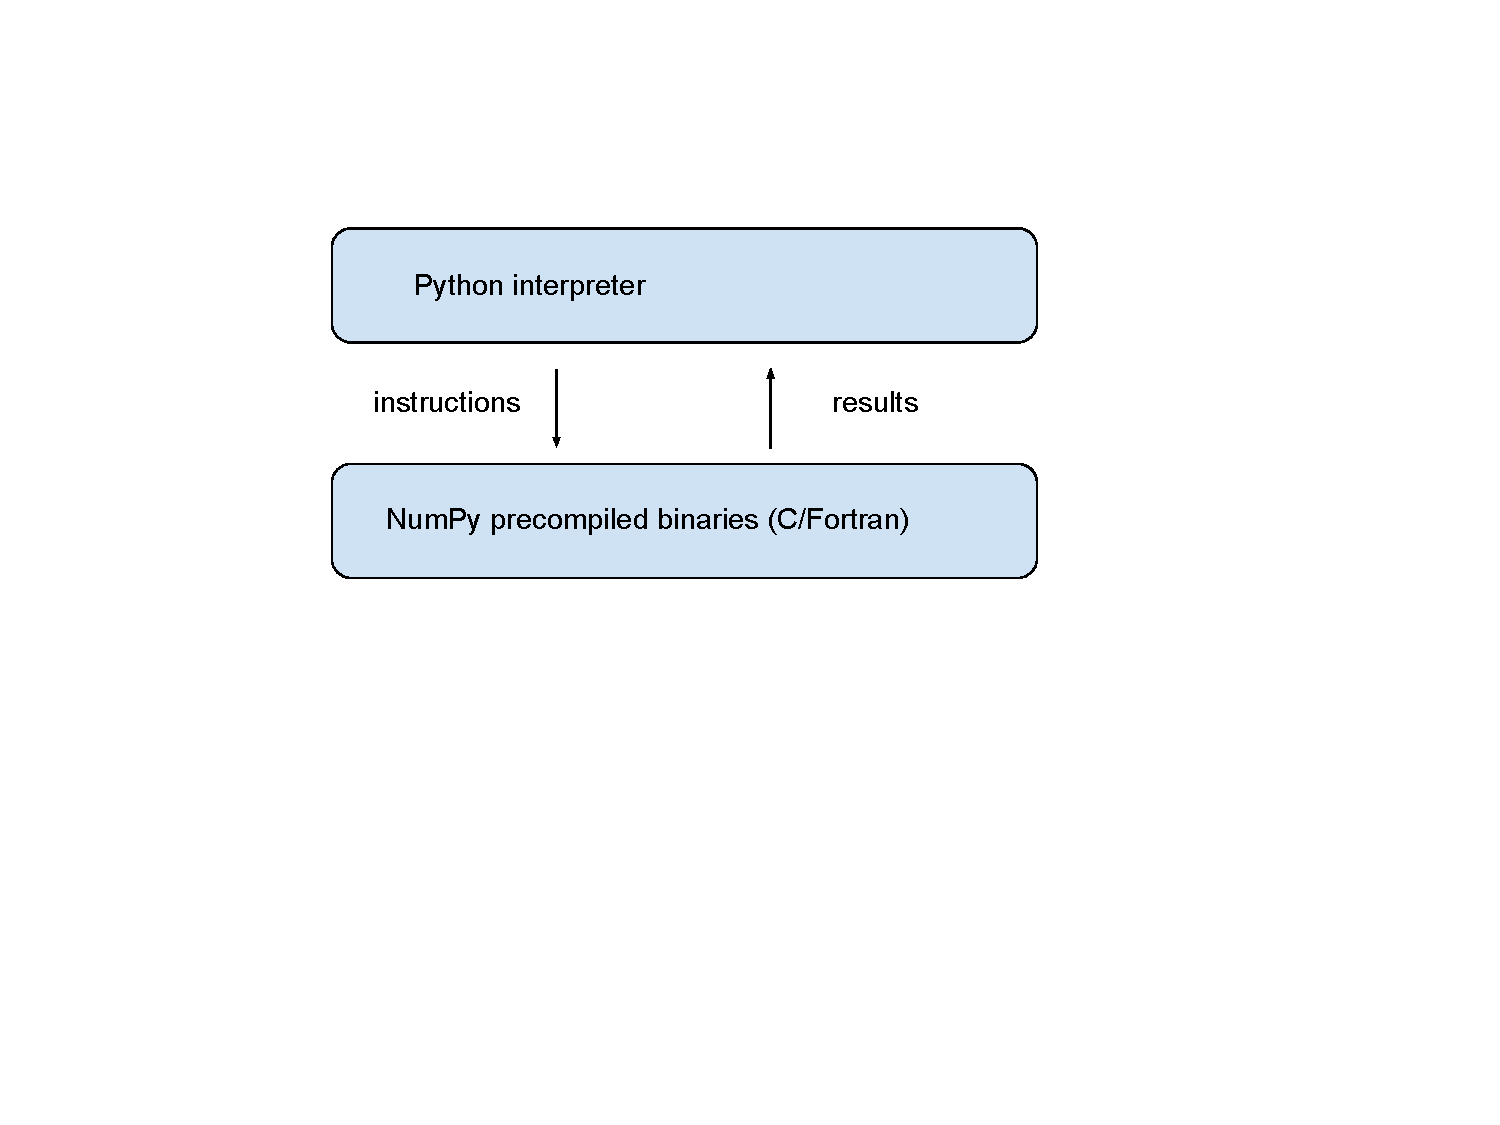
\includegraphics[trim={2cm 8cm 6cm 3cm},clip]{numpy.pdf}}
       \end{center}
    \end{figure}

    \begin{itemize}
        \item Key is converting problems to array-processing operations
    \end{itemize}

\end{frame}

\begin{frame}[fragile]

    \begin{minted}{python}
        import numpy 

        A = ((2.0, -1.0),
             (5.0, -0.5))

        b = (0.5, 1.0)

        A, b = np.array(A), np.array(b)

        x = np.inv(A) @ b
    \end{minted}

\end{frame}



\begin{frame}
    \frametitle{MATLAB}

    NumPy is similar to and borrows from the older MATLAB programming
    environment

    \vspace{0.5em}
    \vspace{0.5em}
    \begin{figure}
       \begin{center} % l b r t
        \scalebox{.6}{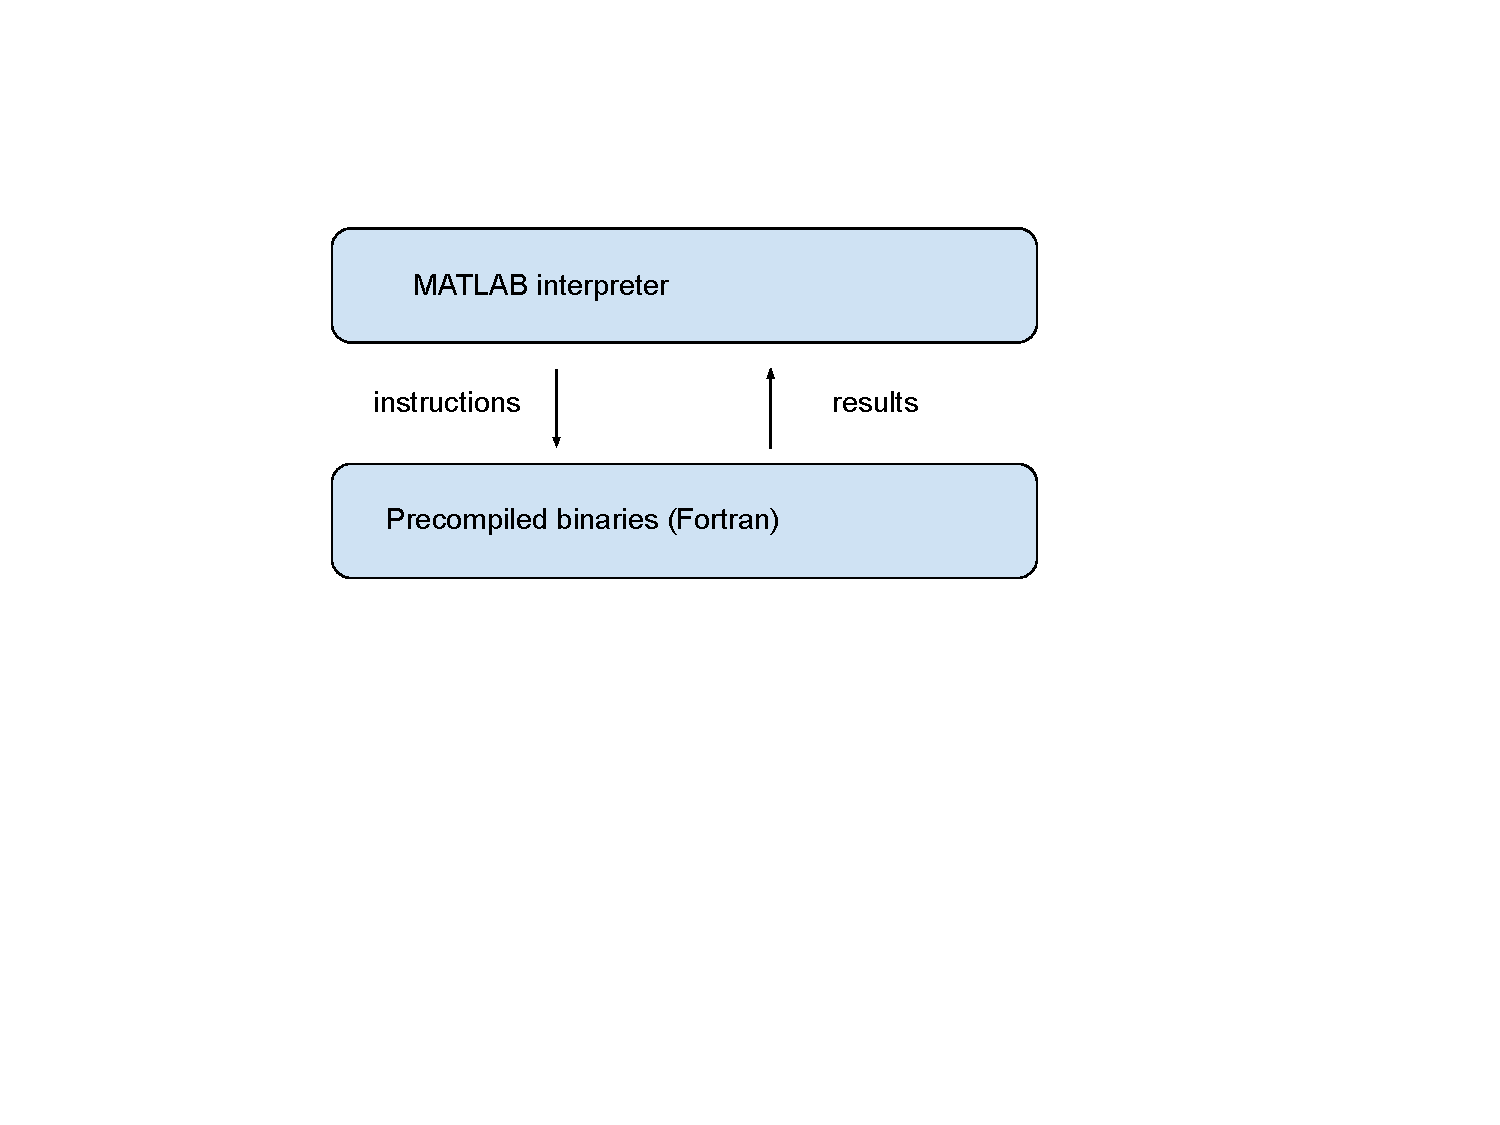
\includegraphics[trim={2cm 8cm 6cm 3cm},clip]{matlab.pdf}}
       \end{center}
    \end{figure}


\end{frame}



\begin{frame}[fragile]

    Here
    %
    \begin{enumerate}
        \item arrays are built in a high-level interface
        \item execution takes place in an efficient low-level environment
        \item results are returned to the high-level interface
    \end{enumerate}
    
    \begin{minted}{matlab}
        A = [2.0, -1.0
             5.0, -0.5];

        b = [0.5, 1.0]';

        x = inv(A) * b
    \end{minted}

    
\end{frame}



\begin{frame}[fragile]
    \frametitle{Julia --- rise of the JIT compilers}

    Can do MATLAB / NumPy style vectorized operations

    \begin{minted}{julia}
A = [2.0  -1.0
     5.0  -0.5]

b = [0.5  1.0]'

x = inv(A) * b
    \end{minted}
    
\end{frame}


\begin{frame}
    
    But also has fast loops via an efficient JIT compiler

    \vspace{0.5em}
    \vspace{0.5em}
    \Eg Suppose, again, that we want to compute 
    %
    \begin{equation*}
        k_{t+1} = s k_t^\alpha + (1 - \delta) k_t
    \end{equation*}
    %
    from some given $k_0$ 


    \vspace{0.5em}
    \vspace{0.5em}
    \vspace{0.5em}
    \vspace{0.5em}
    \begin{itemize}
        \item Iterative, not easily vectorized
    \end{itemize}

\end{frame}


\begin{frame}[fragile]
    
    \begin{minted}{julia}

function solow(k0, α=0.4, δ=0.1, n=1_000)
    k = k0
    for i in 1:(n-1)
        k = s * k^α + (1 - δ) * k
    end
    return k
end

solow(0.2)
    \end{minted}

    \vspace{0.5em}
    \vspace{0.5em}
    \vspace{0.5em}
    \vspace{0.5em}

    Julia accelerates \texttt{solow} at runtime via a JIT compiler

\end{frame}

\begin{frame}[fragile]
    \frametitle{Python + Numba --- same architecture, same speed}
    
    \begin{minted}{python}
from numba import jit

@jit(nopython=True)
def solow(k0, α=0.4, δ=0.1, n=1_000):
    k = k0
    for i in range(n-1):
        k = s * k**α + (1 - δ) * k
    return k

solow(0.2)
    \end{minted}


    Runs at same speed as Julia / C / Fortran

\end{frame}


\begin{frame}
    \frametitle{Back to JAX}

            \vspace{0.5em}
    \begin{itemize}
        \item \brown{J}ust-in-time compilation
            \vspace{0.5em}
        \item \brown{A}utomatic differentiation
            \vspace{0.5em}
        \item \brown{X}ccelerated linear algebra
    \end{itemize}

            \vspace{0.5em}
            \vspace{0.5em}
    JAX has significant advantages over C / Fortran / NumPy / Julia / Numba /
    etc.

            \vspace{0.5em}
            \vspace{0.5em}
    \pause
    \begin{itemize}
        \item But JAX is not uniformly ``better'' --- discuss later
    \end{itemize}


\end{frame}


\begin{frame}[fragile]
    \frametitle{Just-in-time compilation}
    
    \begin{minted}{python}
@jax.jit
def f(x):
    """
    A function that transforms an array x.
    """
    term1 = 2 * jnp.sin(3 * x) * jnp.cos(x/2)
    term2 = 0.5 * x**2 * jnp.cos(5*x) / (1 + 0.1 * x**2)
    term3 = 3 * jnp.exp(-0.2 * (x - 4)**2) * jnp.sin(10*x)
    term4 = 0.8 * jnp.log(jnp.abs(x) + 1) * jnp.cos(x**2 / 8)
    return term1 + term2 + term3 + term4 
    \end{minted}

            \vspace{0.5em}
            \vspace{0.5em}
    \begin{itemize}
        \item Compiles at runtime based on specified shape \& data type
    \end{itemize}

\end{frame}

\begin{frame}[fragile]
    \frametitle{Automatic differentiation}
    
    \vspace{-1em}
    \begin{minted}{python}
import jax.numpy as jnp
from jax import grad, jit

def f(θ, x):
  for W, b in θ:
    w = x @ W + b
    x = jnp.tanh(w)  
  return x

def loss(θ, x, y):
  return jnp.sum((y - f(θ, x))**2)

grad_loss = jit(grad(loss))  # Now use gradient descent 
    \end{minted}

\end{frame}


\begin{frame}[fragile]
    \frametitle{Xccelerated linear algebra}

    Array operations are
    %
    \begin{itemize}
        \item JIT-compiled
    \vspace{0.5em}
        \item automatically parallelized
    \vspace{0.5em}
        \item automatically optimized for and deployed to available hardware
    \end{itemize}
    

\end{frame}


\begin{frame}
    
    Advantages over NumPy / MATLAB

    \vspace{0.5em}
    \begin{itemize}
        \item Can specialize machine code to data types \textbf{and} shapes!
        \vspace{0.5em}
        \vspace{0.5em}
        \vspace{0.5em}
        \item Automatically matches tasks with accelerators (GPU / TPU)
        \vspace{0.5em}
        \vspace{0.5em}
        \vspace{0.5em}
        \item Fuses array operations for speed and memory efficiency
    \end{itemize}

\end{frame}

\begin{frame}

    Advantages of JAX (vs PyTorch / Tensorflow / etc.) for economists:
    %
    \begin{itemize}
        \item exposes low level functions
            \vspace{0.5em}
        \item elegant functional programming style -- close to maths
            \vspace{0.5em}
        \item elegant autodiff tools
            \vspace{0.5em}
        \item array operations follow standard NumPy API
            \vspace{0.5em}
        \item automatic parallelization
            \vspace{0.5em}
        \item same code, multiple backends (CPUs, GPUs, TPUs)
    \end{itemize}

\end{frame}

\begin{frame}{Features of JAX}

    Let's look at some useful features
    
\end{frame}

\begin{frame}
    \frametitle{Functional Programming}
    
    JAX adopts a \emp{functional programming style}

    \vspace{0.5em}
    \vspace{0.5em}
    \vspace{0.5em}
    \vspace{0.5em}
    Key feature: Functions are pure

    \begin{itemize}
        \item Deterministic: same input $\implies$ same output 
        \item Have no side effects (don't modify state outside their scope)
    \end{itemize}

\end{frame}


\begin{frame}[fragile]

    A non-pure function

    \begin{minted}{python}
tax_rate = 0.1  # Global 
price = 10.0    # Global

def add_tax_non_pure():
    global price                
    # The next line both accesses and modifies global state
    price = price * (1 + tax_rate)    
    return price 
    \end{minted}
    
\end{frame}


\begin{frame}[fragile]

    A pure function

    \begin{minted}{python}

def add_tax_non_pure(price, tax_rate=0.1):
    price = price * (1 + tax_rate)    
    return price 
    \end{minted}
    
\end{frame}


\begin{frame}

    General advantages:

    \begin{itemize}
        \item Helps testing: each function can operate in isolation
        \item Data dependencies are explicit, which helps with understanding and optimizing complex computations 
        \item Promotes deterministic behavior and hence reproducibility
        \item Prevents subtle bugs that arise from mutating shared state
    \end{itemize}

\end{frame}



\begin{frame}
    
    Advantages for JAX:

     \begin{itemize}
         \item Functional programming facilitates autodiff because
             pure functions are more straightforward to differentiate (don't mod
             external state
         \item Pure functions are easier to
             parallelize and optimize for hardware accelerators like GPUs (don't
             depend on shared mutable state, more independence)
         \item Transformations can be composed cleanly with multiple
             transformations yielding predictable results
        \item Portability across hardware: The functional approach helps JAX
            create code that can run efficiently across different hardware
            accelerators without requiring hardware-specific implementations.
     \end{itemize}


\end{frame}

\begin{frame}
    \frametitle{JAX PyTrees}

    A PyTree is a concept in the JAX library that refers to a tree-like data structure built from Python containers.

    \Egs

    \begin{itemize}
        \item A dictionary of lists of parameters
        \item A list of dictionaries of parameters, etc.
    \end{itemize}

    JAX can

    \begin{itemize}
        \item apply functions to all leaves in a PyTree structure
        \item differentiate functions with respect to the leaves of PyTrees
        \item etc.
    \end{itemize}

\end{frame}


\begin{frame}
    
    
    \resizebox{1.0\textwidth}{!}{
        % JAX PyTree TikZ Diagram with Pygments Syntax Highlighting
% To use this in your LaTeX document:
% 1. Ensure you have the required packages in your preamble: tikz, minted, varwidth
% 2. Load TikZ libraries: shapes, arrows, positioning, fit, backgrounds, calc
% 3. Define the colors and minted settings in your preamble
% 4. Place this code inside a figure environment

% Required packages for your preamble:
% \usepackage{tikz}
% \usepackage{minted}
% \usepackage{varwidth}
% \usetikzlibrary{shapes,arrows,positioning,fit,backgrounds,calc}

% Color definitions for your preamble:
% \definecolor{containerblue}{RGB}{66, 133, 244}
% \definecolor{leafgreen}{RGB}{52, 168, 83}
% \definecolor{textgray}{RGB}{51, 51, 51}
% \definecolor{backgroundgray}{RGB}{248, 249, 250}
% \definecolor{codebg}{RGB}{241, 241, 241}

% Minted settings for your preamble:
% \setminted[python]{
%   fontsize=\small,
%   baselinestretch=1.2,
%   bgcolor=codebg,
%   linenos=false,
%   breaklines=true,
%   frame=none
% }

% Place the following code in your document inside a figure environment:
% \begin{figure}
%   \centering
%   ... code below ...
%   \caption{JAX PyTree Structure Visualization}
%   \label{fig:jax-pytree}
% \end{figure}

\begin{tikzpicture}[
    % Node styles
    container/.style={draw=containerblue!70!black, fill=containerblue, rounded corners=3pt, minimum width=3cm, minimum height=1cm, text=white, font=\sffamily\bfseries},
    leaf/.style={draw=leafgreen!70!black, fill=leafgreen, rounded corners=3pt, minimum width=2cm, minimum height=1cm, text=white, font=\sffamily\bfseries},
    label/.style={font=\sffamily\small, text=textgray},
    level distance=2cm,
    sibling distance=3cm
]

% Background
\node[rectangle, fill=backgroundgray, minimum width=20cm, minimum height=15cm] (background) at (0,0) {};

% Title
\node[font=\sffamily\bfseries\Large, text=textgray] at (0,6.5) {JAX PyTree Structure};

% Sample code with syntax highlighting
\node[anchor=north] (code) at (0,5.5) {
  \begin{varwidth}{14cm}
    \begin{minted}{python}
pytree = {
    "a": [1, 2, 3],
    "b": {"c": jnp.array([4, 5]), "d": jnp.array([[6, 7], [8, 9]])}
}
    \end{minted}
  \end{varwidth}
};

% Add a border around the code
\begin{scope}[on background layer]
\draw[rounded corners=3pt, draw=black!20] 
  ([shift={(-0.5em,-0.5em)}]code.south west) rectangle 
  ([shift={(0.5em,0.5em)}]code.north east);
\end{scope}

\path (code.south) -- ++(0,-1.5) coordinate (after_code);

\node[container] (root) at (0,2) {dict};

% First level children
\node[container] (list) at (-4,1) {list};
\node[label] at (-4,1.8) {"a"};
\node[container] (dict) at (4,1) {dict};
\node[label] at (4,1.8) {"b"};

% Second level - list elements
\node[leaf] (n1) at (-6,-1) {1};
\node[leaf] (n2) at (-4,-1) {2};
\node[leaf] (n3) at (-2,-1) {3};

% Second level - dict elements
\node[container] (array1) at (2,-1) {array};
\node[label] at (2,-0.2) {"c"};
\node[container] (array2) at (6,-1) {array};
\node[label] at (6,-0.2) {"d"};

% Array values (leaf nodes)
\node[leaf, text width=2.5cm, align=center] (val1) at (2,-3) {[4, 5]};
\node[leaf, text width=3cm, align=center] (val2) at (6,-3) {[[6, 7], [8, 9]]};

% Edges connecting nodes
\draw[->, >=stealth, thick, textgray] (root) -- (list);
\draw[->, >=stealth, thick, textgray] (root) -- (dict);
\draw[->, >=stealth, thick, textgray] (list) -- (n1);
\draw[->, >=stealth, thick, textgray] (list) -- (n2);
\draw[->, >=stealth, thick, textgray] (list) -- (n3);
\draw[->, >=stealth, thick, textgray] (dict) -- (array1);
\draw[->, >=stealth, thick, textgray] (dict) -- (array2);
\draw[->, >=stealth, thick, textgray] (array1) -- (val1);
\draw[->, >=stealth, thick, textgray] (array2) -- (val2);

% Legend
\node[container, minimum width=1cm, minimum height=0.6cm] (legend1) at (-7,-5) {};
\node[text=textgray, font=\sffamily, anchor=west] at (-6.5,-5) {Container nodes (dict, list, tuple)};

\node[leaf, minimum width=1cm, minimum height=0.6cm] (legend2) at (-7,-6) {};
\node[text=textgray, font=\sffamily, anchor=west] at (-6.5,-6) {Leaf nodes (arrays, scalars)};

% Additional explanation
\node[text=textgray, font=\sffamily\bfseries, align=center] at (0,-4.5) {JAX PyTrees: Nested containers with leaves as arrays or scalars};

\end{tikzpicture}

    }

\end{frame}


\begin{frame}[fragile]
    
    \begin{minted}{python}
# Apply gradient updates to all parameters
def sgd_update(params, grads, learning_rate):
    return jax.tree_map(
        lambda p, g: p - learning_rate * g, 
        params, 
        grads
    )

# Calculate gradients (PyTree with same structure as params)
grads = jax.grad(loss_fn)(params, inputs, targets)

# Update all parameters at once
updated_params = sgd_update(params, grads, 0.01)    
    \end{minted}

\end{frame}



\end{document}
